\documentclass[tikz,border=5pt]{standalone}
\usepackage{luatexja}
\usepackage[hiragino-pron]{luatexja-preset}
\usepackage{amsmath,amssymb}
\usepackage{pgfplots}
\pgfplotsset{compat=1.18}
\usetikzlibrary{arrows.meta,calc,decorations.markings,patterns,positioning}

% Common styles
\tikzset{
  axis/.style={-{Stealth[length=6pt]}, thick},
  curve/.style={thick, red},
  dashed curve/.style={thick, dashed, blue},
  dot/.style={circle, fill, inner sep=1.5pt},
  open dot/.style={circle, draw, fill=white, inner sep=1.5pt},
}

\begin{document}
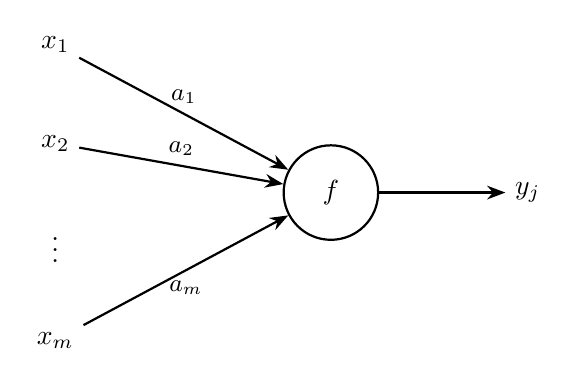
\begin{tikzpicture}[
  neuron/.style={circle, draw, minimum size=1.2cm, thick},
  >=Stealth
]
  % Input nodes
  \node (x1) at (0, 2.5) {$x_1$};
  \node (x2) at (0, 1.25) {$x_2$};
  \node (xdots) at (0, 0) {$\vdots$};
  \node (xm) at (0, -1.25) {$x_m$};

  % Neuron
  \node[neuron] (f) at (3.5, 0.625) {$f$};

  % Output
  \node (yj) at (6, 0.625) {$y_j$};

  % Connections with weights
  \draw[->, thick] (x1) -- (f) node[midway, above, font=\small] {$a_1$};
  \draw[->, thick] (x2) -- (f) node[midway, above, font=\small] {$a_2$};
  \draw[->, thick] (xm) -- (f) node[midway, below, font=\small] {$a_m$};

  % Output arrow
  \draw[->, thick] (f) -- (yj);
\end{tikzpicture}
\end{document}
